\begin{figure}[htbp]
\centering
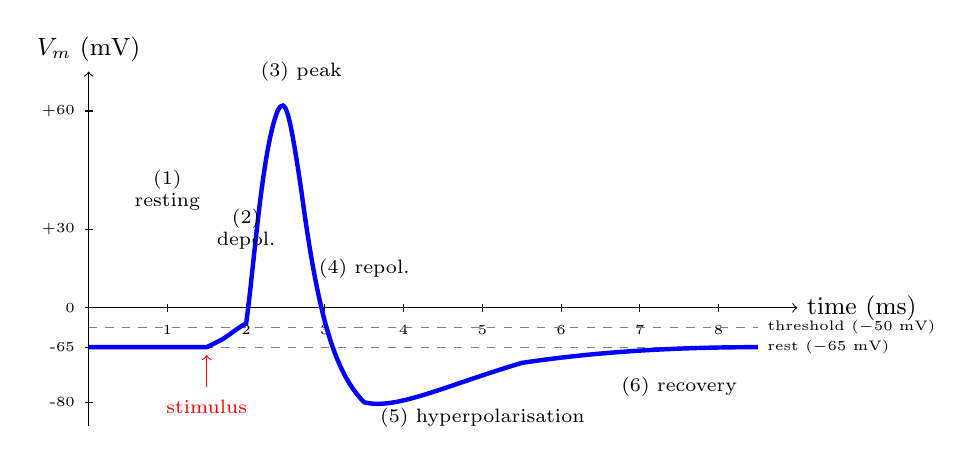
\begin{tikzpicture}[scale=1.0, every node/.style={font=\small}]
  % Axes
  \draw[->] (0,0) -- (9.0,0) node[right] {time (ms)};
  \draw[->] (0,-1.5) -- (0,3.0) node[above] {$V_m$ (mV)};
  % Tick marks x
  \foreach \x/\t in {1/1, 2/2, 3/3, 4/4, 5/5, 6/6, 7/7, 8/8} {
    \draw (\x,-0.05) -- (\x,0.05);
    \node[below] at (\x,-0.1) {\tiny \t};
  }
  % Tick marks y
  \foreach \y/\t in {-1.2/-80, -0.5/-65, 0/0, 1.0/+30, 2.5/+60} {
    \draw (-0.05,\y) -- (0.05,\y);
    \node[left] at (-0.05,\y) {\tiny \t};
  }
  % Threshold line
  \draw[dashed, color=gray] (0,-0.25) -- (8.5,-0.25);
  \node[right, font=\tiny] at (8.5,-0.25) {threshold ($-50$ mV)};
  % Resting line
  \draw[dashed, color=gray] (0,-0.5) -- (8.5,-0.5);
  \node[right, font=\tiny] at (8.5,-0.5) {rest ($-65$ mV)};
  % Action potential trace
  \draw[ultra thick, blue]
    (0,-0.5)
    .. controls (1.0,-0.5) and (1.4,-0.5) .. (1.5,-0.5)
    -- (1.7,-0.4)
    .. controls (1.85,-0.3) and (1.9,-0.25) .. (2.0,-0.2)
    .. controls (2.1,0.5) and (2.2,2.0) .. (2.4,2.5)
    .. controls (2.5,2.7) and (2.55,2.5) .. (2.7,1.5)
    .. controls (2.9,0.0) and (3.1,-0.8) .. (3.5,-1.2)
    .. controls (3.9,-1.3) and (4.5,-1.0) .. (5.5,-0.7)
    .. controls (6.5,-0.55) and (7.5,-0.5) .. (8.5,-0.5);
  % Phase annotations
  \node[align=center, font=\scriptsize] at (1.0,1.5) {(1)\\resting};
  \node[align=center, font=\scriptsize] at (2.0,1.0) {(2)\\depol.};
  \node[align=center, font=\scriptsize] at (2.7,3.0) {(3) peak};
  \node[align=center, font=\scriptsize] at (3.5,0.5) {(4) repol.};
  \node[align=center, font=\scriptsize] at (5.0,-1.4) {(5) hyperpolarisation};
  \node[align=center, font=\scriptsize] at (7.5,-1.0) {(6) recovery};
  % Stimulus arrow
  \draw[->, color=red] (1.5,-1.0) -- (1.5,-0.6);
  \node[below, color=red, font=\scriptsize] at (1.5,-1.05) {stimulus};
\end{tikzpicture}
\caption[Action potential cycle]{The six phases of the action potential:
(1)~resting at $-65\,\text{mV}$ with closed voltage-gated channels;
(2)~depolarisation as voltage-gated sodium channels open;
(3)~peak near $+30\,\text{mV}$;
(4)~repolarisation as sodium channels inactivate and potassium channels
open; (5)~hyperpolarisation overshoot below resting; (6)~recovery to
rest as potassium channels close. The absolute refractory period
spans phases (3) through early (4); the relative refractory period
extends through (5) and (6).}
\label{fig:vol06:ch07:ap-cycle}
\end{figure}
